Refer to the data for the world's 10 largest companies in Exercise 1.4. Construct a chi-square plot using all \textit{three} variables. The chi-square quantiles are
\newline
0.3518 \ 0.7978 \ 1.2125 \ 1.6416 \ 2.1095 \ 2.6430 \ 3.2831 \ 4.1083 \ 5.3170 \ 7.8147

\begin{figure}[H]
    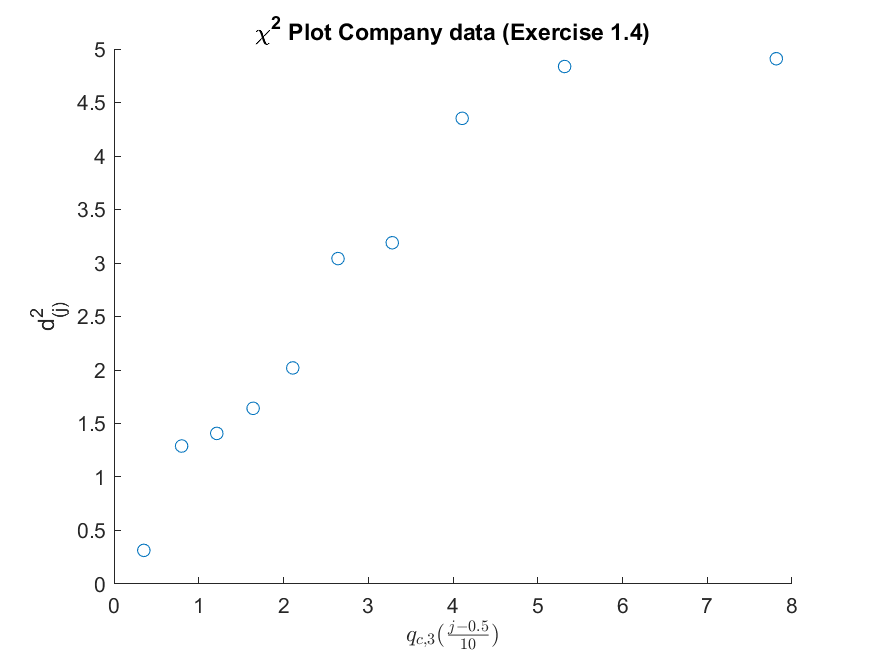
\includegraphics[scale=0.8]{./matlab/chapter-4/sol4.25.png}
\end{figure}

\begin{center}
    \begin{tabular}{ccc}
        \hline % chktex 44
        $j$ & $d_{(j)}^{2}$ & $q_{c, 3}\left(\frac{j-\frac{1}{2}}{10}\right)$ \\
        \hline % chktex 44
        1 & 0.3142 & 0.3518 \\
        2 & 1.2894 & 0.7978 \\
        3 & 1.4073 & 1.2125 \\
        4 & 1.6418 & 1.6416 \\
        5 & 2.0195 & 2.1095 \\
        6 & 3.0411 & 2.6430 \\
        7 & 3.1891 & 3.2831 \\
        8 & 4.3520 & 4.1083 \\
        9 & 4.8364 & 5.3170 \\
       10 & 4.9090 & 7.8147 \\
       \hline % chktex 44
    \end{tabular}
\end{center}
